\documentclass[a4paper]{article}


\usepackage{alphabeta} 
\usepackage{enumitem} 
\usepackage{mathtools}
\usepackage{amsmath, amssymb} 
\usepackage{amsthm}
\usepackage{cancel} 
\usepackage[margin=0.70in]{geometry} 
\geometry{left=3cm,right=3cm,top=2.4cm,bottom=2.4cm}	%the page geometry as defined, A4=210x297mm
\usepackage{graphicx}
\usepackage{wrapfig}
\usepackage{caption}
\usepackage{textcomp}
\usepackage{tabto}
\usepackage{layout}
\usepackage{bm}
\usepackage{minipage-marginpar}
\usepackage[dvipsnames]{xcolor}
\usepackage{hyperref}
\usepackage{dutchcal}
\usepackage{derivative}
\usepackage{esint}
%\usepackage{biblatex}
\usepackage{subcaption}
\usepackage{booktabs}\usepackage{derivative}
\usepackage[flushleft]{threeparttable}
\usepackage[capbesideposition=outside,capbesidesep=quad]{floatrow}
\usepackage{derivative}
\usepackage[thinc]{esdiff}
%%RENEW

\newtheorem{problem}{Άσκηση}
\newtheorem*{solution*}{Λύση}
\newtheorem{definition}{Ορισμός}[subsection]
\newtheorem{properties}{Ιδιότητες}[subsection]
\newtheorem{theorem}{Θεώρημα}[subsection]
\newtheorem{protash}{Πρόταση}[subsection]
\newtheorem{porisma}{Πόρισμα}[subsection]
\newtheorem{lemma}{Λήμμα}[subsection]
\newtheorem*{prooof}{Απόδειξη}
\newtheorem*{notes}{Παρατηρήσεις}
\newtheorem*{note}{Παρατήρηση}
\newtheorem*{app}{Εφαρμογή} 
\newtheorem*{example}{Παράδειγμα}
\newtheorem*{examples}{Παραδείγματα}


\newcommand\numberthis{\addtocounter{equation}{1}\tag{\theequation}}
%\renewcommand{\labelenumi}{\roman{enumi}}
\newcommand{\approxtext}[1]{\ensuremath{\stackrel{\text{#1}}{\approx}}}
\renewcommand{\figurename}{Εικόνα.}
\renewcommand{\tablename}{Πίνακας.}
%\renewcommand\refname{New References Header}
\renewcommand*\contentsname{Περιεχόμενα}
%\DeclareDerivative{\odv}{\mathrm{d}}


\begin{document}
\begin{titlepage}			%makes a title page. Remember to change the author, CID, username and group number to what is appropriate for you!
	\centering
	{\scshape\LARGE Εθνικό Μετσόβιο Πολυτεχνείο\par}
	{\scshape \LARGE Σ.Ε.Μ.Φ.Ε.\par}
	\vspace{1cm}
	{\huge\bfseries Θερμιονική Εκπομπή Ηλεκτρονίων \par}
	\vspace{1cm}
	{\Large\itshape Θωμόπουλος Σπύρος\par}		%remember to change these!
	
	%		{\large Group \@group\unskip\strut\par}
	{\large A.M ge19042 \hfill \\ E-mail spyros.thomop@gmail.com \\}%ge19042@mail.ntua.gr\par		%remember to change these!
	\vspace{1cm}
	{\large Ημερμονηνία Παράδοσης 26/11/2021\par}
\end{titlepage}


\newpage 

\subsection*{Σκοπός}
Ο στόχος της εν λόγω εργαστηριακής άσκησης είναι η μελέτη του φαινομένου της θερμιονικής εκπομπής ηλεκτρονίων από την επιφάνεια μετάλλου. Θα ελεγχθούν δύο νόμοι που το διέπουν, οι νόμοι του Langmuir και του Richardson.

\subsection*{Θεωρητικά Στοιχεία}
\subsubsection*{Μοντέλο Μετάλλου}
Για τα μέταλλα θα χρησιμοποιήσουμε το μοντέλο των ελεύθερων ηλεκτρονίων, σύμφωνα με το οποίο, τα ηλεκτρόνια του μετάλλου που προκαλούν την ηλεκτρική του αγωγιμότητα είναι ελεύθερα, μη αλληλεπιδρώντα και σε πρώτη φάση περιλαμβάνει το γεγονός ότι έχουν διακριτές ενέργειες και ότι είναι φερμιόνια, δηλαδή ακολουθούν την στατιστική Fermi-Dirac και υπόκεινται στην απαγορευτική Αρχή Pauli. 

Θεωρούμε τα ηλεκτρόνια ως επίπεδα κύματα τα οποία ανακλώνται μόνο στο εσωτερικό της επιφάνειάς του. Έτσι παίρνουμε τις δέσμιες καταστάσεις, που σημαίνουν διακριτότητα για την ενέργεια.
% Οι εν λόγω καταστάσεις χαρακτηρίζονται από μεγάλη πυκνότητα και γι' αυτό μπορούμε να θεωρήσουμε το φάσμα της ενέργειας συνεχές.
Επίσης, εξαιτίας της απαγορευτικής αρχής του Pauli, τα ηλεκτρόνια στην θερμοκρασία $T=0K$ δεν βρίσκονται σε ακινησία, αλλά μόνο ένα ζεύγος από αυτά δύναται να καταλάβει την χαμηλότερη ενεργειακή στάθμη. Τα υπόλοιπα λαμβάνουν ενέργειες που ανήκουν σε διακριτές στάθμες οι οποίες γίνονται όλο και πιο πυκνές καθώς πλησιάζουμε πρός το άνω φράγμα τους, την ενέργεια Fermi. 

%θα υπάρχει ένα άνω φράγμα για την 
%%\textcolor{red}{απόλυτη} 
%τιμή της ενέργειας που μπορούν να έχουν τα ηλεκτρόνια εντός του μετάλλου, που καλείται \textit{ενέργεια Fermi, $E_f$}. 



\begin{wrapfigure}{r}{0.4\textwidth}
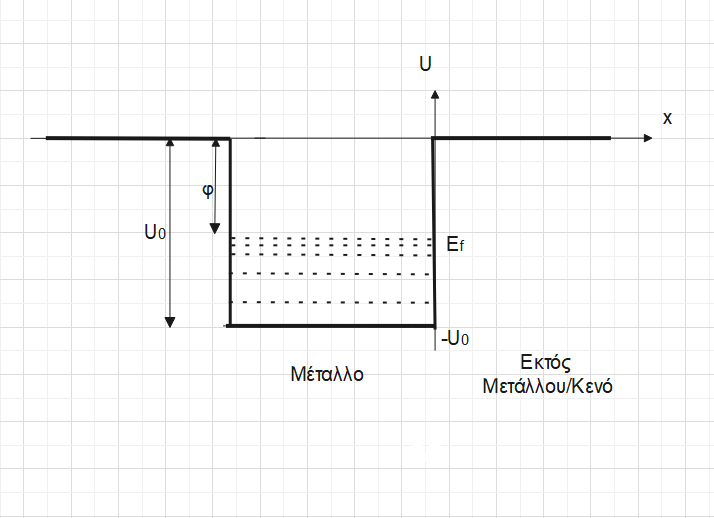
\includegraphics[width=1.0\linewidth]{metal.png} 
\caption{ }
\label{fig:wrapfig}
\end{wrapfigure}
Μπορούμε να θεωρήσουμε το δυναμικό του μετάλλου $-V_0$ και το δυναμικό εκτός μετάλου $0$ (πηγάδι δυναμικού), τότε η ενέργεια Fermi είναι αρνητική, προκειμένου οι υπόλοιπες στάθμες να έχουν 
%\textcolor{red}{κατ' απόλυτη τιμή} 
μικρότερη ενέργεια 
%αλλά η ενέργεια για την οποία το ηλεκτροόνιο εξέρχεται από το μέταλλο να 'ναι μηδενική,
(Εικόνα 1).
%\footnote{Στην πραγματικότητα δεν πρόκειται για σκαλοπάτι δυναμικού όπως φαίνεται στην εικόνα, αλλά για πηγάδι, διότι έτσι επιτυγχάνονται οι δέσμιες καταστάσεις.}
 Η ενέργεια Fermi δίνεται από την σχέση 
 \begin{equation}\label{1}
 	E_f =\textcolor{red}{-} \frac{h^2(3\pi^2 n)^{2/3}}{8m_e\pi^2}
 \end{equation}
όπου n είναι ο αριθμός ηλεκτονίων ανά μονάδα όγκου.

Γενικα, είναι γνωστό από την Μηχανική, ότι σε εναν στοιχειώδη όγκο dV ενός δεδομένου στερεού θα υπάρχει μία στοιχειώδης ποσότητα μάζας dm, ποσότητες που συνδέονται μέσω της πυκνότητας μάζας του στερεού $\rho(r)$, με τον εξής τρόπο: $dm=\rho(r) dV$.
%, όπου $\rho$ είναι η πυκνότητα μάζας του στερεού, μιά συνάρτηση της θέσης, r.
 Κατ' αναλογία, έχουμε ότι σε μία συγκεκριμένη στοιχιώδη περιοχή ενεργειών, πλάτους dE ( δηλαδή για ενέργειες που ανήκουν στο διάστημα $(E,E+dE)$) θα υπάρχει συγκεκριμένος αριθμός ηλεκτρονίων $dN$, που έχουν ενέργεια εντός του $(E,E+dE)$. Τα δύο αυτά μεγέθη συνδέονται μέσω της \textit{πυκνότητας ενεργειακών καταστάσεων} $\rho (E)$, σύμφωνα με την σχέση $dN=\rho(E)dV$. Ωστόσο, επειδή τα ηλεκτρόνια είναι φερμιόνια συνεπώς ακολουθούν την στατιστική Fermi-Dirac, το σύστημα δεν είναι ισοπίθανο να βρίσκεται σε κάθε ενεργειακή κατάσταση. Η κατανομή πιθανότητας δίνεται από την κατανομή Fermi-Dirac $f(E)$, δηλαδή έχουμε ότι $dN=\rho(E)f(E)dV$. Σε άλλη μορφή, έπειτα από την αντικατάσταση της συνάρτησης κατανομής $f(E)$, γράφεται: 
\begin{equation}\label{2}
dN=\rho(E)f(E) = \frac{8\pi}{h^3}\sqrt{2m_e^3}\frac{\sqrt{E}dE}{e^{(E-|E_f|)/kT}+1}
\end{equation}



Ακόμη, δεν έχει γίνει ξεκάθαρος ο λόγος για τον οποίον θεωρούμε την ενέργεια Fermi αρνητική. Προκειμένου να ξεφύγουν τα ηλεκτρόνια απ' το πηγάδι δυναμικού, 
θα πρέπει να έχουν μεγαλύτερη ενέργεια από το ύψος του, πράγμα αδύνατο καθώς είναι παγιδευμένα μεσα στο μέταλλο. Ωστόσο, μπορούμε να τα απεγκλωβίσουμε, είτε προσφέροντάς τους ενέργεια φ (έργο εξόδου), ώστε να υπερπηδήσουν το πηγάδι, είτε αν με κάποιον τρόπο μετατρέψουμε το πλάτος του σκαλοπατιού από άπειρο σε πεπερασμένο (φράγμα δυναμικού). Η δεύτερη περίπτωση αναφέρεται στο φαινόμενο της ψυχρής εκπομπής το οποίο εξηγείται με βάση το κβαντομηχανικό φαινόμενο σήραγγας. Η πρώτη σχετίζεται με το φαινένο θερμιονικής εκπομπής, όταν η υπολειπόμενη ενέργεια (έργο εξαγωγής) προσφέρεται στα ηλεκτρόνια μέσω της θέρμανσής τους, η οποία στην περίπτωσή μας θα προκληθεί από την εφαρμογή συνεχούς ηλεκτρικού ρεύματος σε μία πλάκα μετάλλου.
\footnote{Υπάρχουν και άλλοι τρόποι για να λάβουν τα ηλεκτρόνια την απαιτούμενη ενέργεια ώστε να εξέλθουν απ΄ το μέταλλό, όπως για παράδειγμα από Η/Μ ακτινοβολία και από προσπίπτωντα ιόντα ή ηλεκτρόνια.} 
Άρα για τις ενέργειες ισχύει η σχέση:
\begin{align*}\label{3}
U_0 = E_f + \phi \numberthis
\end{align*}

%
%\textcolor{red}{Πρέπει να σημειωθεί πως εξαιτίας της κβαντομηχανικής θα υπάρχει ένα ποσοστό από τα ηλεκτρόνια που "δικαιούνται" να εξέλθουν (τους έχει προσφερθεί έργο φ), τα οποία θα ανακλώνται από το δυναμικό. Αυτό το ποσοστό εκφράζεται από τον μέσο συντελεστή ανάκλασης D.}

Αριθμητικά, για το βολφράμιο που θα χργσιμοποιηθεί στην πειραματική διαδικασία, η ενέργεια Fermi είναι $|E_f|=5.7eV$ ενώ το έργο εξαγωγής, η ενέργεια δηλαδή που πρέπει να προσφέρουμε στο ηλεκτρόνιο για ξεπεράσει το δυναμικό του μετάλλου είναι $\phi=4.5eV$. Υποθετικά, αν τα ηλεκτρόνια δεν είχαν ενέργεια, τότε θα  βρίσκονταν στο δυναμικό του μετάλλου $V_0=-(5.7+4.5)=-10.2V$. Ωστόσο, αυτό είναι αδύνατο και τους "επιβάλλεται" μια ελάχιστη ενέργεια εώς $E_f=5.7eV$ άρα 
η ενέργειά τους δύναται να φτάσει εώς $E'=-10.2eV+5.7eV=-4.5eV$, απ' όπου για να φτάσουν στο μηδενικό δυναμικό/μηδενική ενέργεια θα πρέπει να τους προσφερθεί επιπλέον ενέργεια μεγαλύτερ ή ίση με το έργο εξαγωγής φ. Ο προσδιορισμός του φ είναι ένας από τους πειραματικούς μας στόχους.

\subsubsection*{Το φαινόμενο της θερμιονικής εκπομπής}
\begin{wrapfigure}{r}{0.4\textwidth}
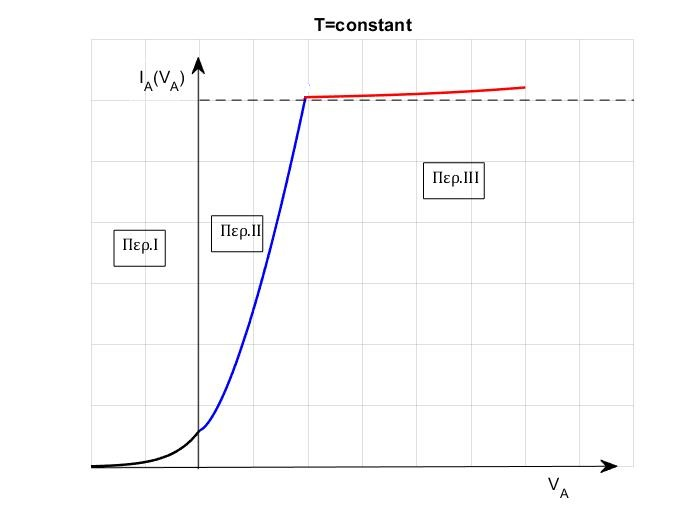
\includegraphics[width=1.0\linewidth]{i(v).jpg} 
\caption{ }
\label{fig:wrapfig}
\end{wrapfigure}
Έστω ότι σε περιοχή υψηλού κενού έχουμε τοποθετήσει έναν μεταλλικό αγωγό, τον οποίο θερμαίνουμε. Τότε, σε μερικά από τα ελεύθερα ηλεκτρόνιά του προσδίδεται το απαιτούμενο ποσό ενέργειας (έργο εξαγωγής) έτσι ώστε να εξέλθουν από την θερμή επιφάνειά του. Ο αγωγός - πηγή ηλεκτρονίων καλείται \textit{κάθοδος}. 

Τα εξερχόμενα ηλεκτρόνια δημιουργούν ένα θερμό νέφος ηλεκτρονίων γύρω απ' την επιφάνεια του αγωγού. Ένα μέρος του νέφους μπορεί συλλεχθεί και να μεταφραστεί ως ηλεκτρικό ρεύμα, από έναν άλλον αγωγό τον οποίο τοποθετούμε απέναντι από την κάθοδο. 

Ο αγωγός - συλλέκτης ηλεκτρονίων καλέιται \textit{άνοδος}, το ρεύμα που δημιουργείται \textit{ανοδικό ρεύμα} και το σύστημα καθόδου-ανόδου \textit{δίοδος κενού}.

Η θέρμανση της ανόδου επιτυγχάνεται με έναν θερμαντήρα στον οποίο εφαρμόζουμε συνεχές ηλεκτρικό ρεύμα. Το ανοδικό ρεύμα $I_A$, ανιχνεύεται όταν η διαφορά δυναμικού ανόδου-καθόδου $V_A$, είναι θετική. Η εξάρτηση του $I_A$ από την $V_A$ χωρίζεται σε τρεις βασικές περιοχές


\begin{itemize}
\item[\underline{Περιοχή 1,}]\textit{$V_A<0 $} \\ 
Δεν θα μελετηθεί πειραματικά, αλλά εκεί ανιχνεύεται ανοδικό ρεύμα το οποίο αυξάνεται εκθετικά με την ανοδική τάση $(I_A\sim exp(-V_A/kT))$ και οφείλεται στα ηλεκτρόνια υψηλής ενέργειας που καταφέρνουν να φτάσουν στην άνοδο παρ'ολη την άπωσή τους από αυτή και γι' αυτό είναι αμελητέο, με μέγιστη τιμή $I_A(V_A=0)=I_0$.

\item[\underline{Περιοχή 2,}]\textit{$0<V_A<V_{κορ} $} (νόμος Langmuir / "3/2") \\ 
Σε αυτή την περιοχή ισχύει η μονοδιάσταση εξίσωση Poisson καθώς έχουμε συνεχή κατανομή φορτίων $\rho(x)$, εξαιτίας του ηλεκτρονιακού νέφους 
\begin{equation*}
\odv[2]{U(x)}{x}= -\frac{\rho(x)}{\epsilon_0}\Rightarrow \hdots \Rightarrow J_A = J_0+ \frac{8\epsilon_0}{9r_A\beta^2}\sqrt{\frac{2e}{m}}V_A^{3/2}  
\end{equation*}

όπου $r_A$ η ακτίνα της κυκλικής καθόδου και $\beta=\beta(r_A/r_K)$ μία αδιάστατη σταθερά.
Ο νόμος αυτός για το ρεύμα δίνει 
\begin{equation}\label{4}
I_A = I_0 + B\times V_A^{3/2} \xRightarrow{I_0\simeq0} \boxed{I_A \approx B\times V_A^{3/2}}
\end{equation}

\item[\underline{Περιοχή 3:}]\textit{$V_a>V_{κορ}$} (νόμος Richardson) \\
	Σε αυτή την περιοχή έχουμε κορεσμό, δηλαδή πολύ μικρή μεταβολή του ρεύματος της ανόδου με την αύξηση της ανοδικής τάσης και εντονότερη εξάρτηση από την θερμοκρασία.
	
	 Αν $dN_x$ ο αριθμός των ηλεκτρονίων εντός του μετάλλου με ενέργεια $E\geq E_f+\phi$ (μετά την θέρμανσή του) και ταχύτητα στην περιοχή $(u_x,u_x+du_x)$, τότε, με βάση την σχέση για την πυκνότητα ρεύματος $J_x = eu_x dN$ και την (\ref{2}) καταλήγουμε στην σχέση \footnotemark 
	\begin{equation}\label{5}
	J_A =\underbrace{\frac{4\pi em}{h^3}}_{C}k^2 T^2e^{-\frac{\phi}{kT}}
	\end{equation}
\footnotetext{Για να λάβουμε υπόψιν και το κβαντομηχανικό φαινόμενο κατά το οποίο μέρος των ηλεκτρονίων με μεγαλύτερη ενέργεια από το πηγάδι ανακλώνται μπορούμε να πολλαπλασιάσουμε με (1-D), όπου D ο συντελεστής ανάκλασης. Ωστόσο δεν θα το συμπεριλάβουμε στο μοντέλο του μετάλλου και κατ' επέκταση στην επεξαργασία των μετρήσεων καθώς η συμβολή του είναι ανεπαίσθητη. Ακόμη, στην συνέχεια θα λογαριθμίσουμε την σχέση για να την γραμμικοποιήσουμε και θα προκύψει μία ευθεία από την οποία θα χρειαστούμε την κλίση, ενώ ο συντελεστής ανάκλασης συναντάται στον σταθερό όρο.}	
	
	όπου για το αντίστοιχο ανοδικό ρεύμα γίνεται \footnotemark
	\begin{equation}\label{6}
	I_A = CT^2exp(-\frac{\phi}{kT})
	\end{equation}
	
	\footnotetext{Θα μπορούσαμε επίσης να συμπεριλάβουμε μία ακόμη διόρθωση στο μοντέλο $\phi \rightarrow \phi-\Delta\phi$, όπου  $\Delta\phi$ είναι η μείωση του έργου εξαγωγής λόγω της αλληλεπίδρασης του εξερχόμενου ηλεκτρονίου με τα επαγώμενα +e φορτία στην επιφάνεια του μετάλλου και με το ηλεκτρικό πεδίο που δημιουργεί η ανοδική τάση (φαινόμενο Schottky). Στην περίπτωσή μας είναι $\Delta\phi\simeq0.12eV$.}
\end{itemize}


%στο δυναμικό προστίθεται η αντίστοιχη ποσότητα και γίνεται $V_0' = -10.2V+5.7V=-4.5V$, απ' όπου για να φτάσουν στο μηδενικό δυναμικό θα πρέπει να του προσφερθεί ενέργεια ίση με το έργο εξαγωγής. 
%Αυτό φαίνεται στην Εικόνα 2.b.



\subsection*{Πειραματική Διάταξη }
H πειραματική διάταξη αποτελείται από: 
\begin{itemize}
\item[.] Δίοδο υψηλού κενού. Η κάθοδος είναι φτιαγμένη από λεπτό σύρμα βολφραμίου $(L=70mm,R=0.08mm)$ και πίσω της υπάρχει ένα μεταλλικός δίσκος για να κάνει το ηλεκτρικό πεδίο στην περιοχή μεταξύ των δύο ηλεκτροδίων πιό ομαλό.
\item[.] Τροφοδοτικό απ' το οποίο χρησιμοποιούμε δύο πηγές, μία πηγή σταθεροποιημένου ρεύματος $I_\theta\sim 1-2.5A$ για την θέρμανση της καθόδου και μία για την τροφοδότηση της διόδου με την ανοδική τάση(0-300V DC).
\item[.] Πολύμετρο για την μέτρηση της ανοδικής τάσης $V_A$.
\item[.] Μικροαμπερόμετρο για την μέτρηση του ανοδικού ρεύματος $I_A$.
\item[.] Ψηφιακό αμπερόμετρο μεγάλης ακρίβειας για την μέτρηση του ρεύματος θέρμανσης $I_\theta$ στην κάθοδο.
\end{itemize}
Η συνδεσμολογία του κυκλώματος φαίνεται στην Εικόνα 2.
\begin{figure}[h!]
\centering
\caption{ }
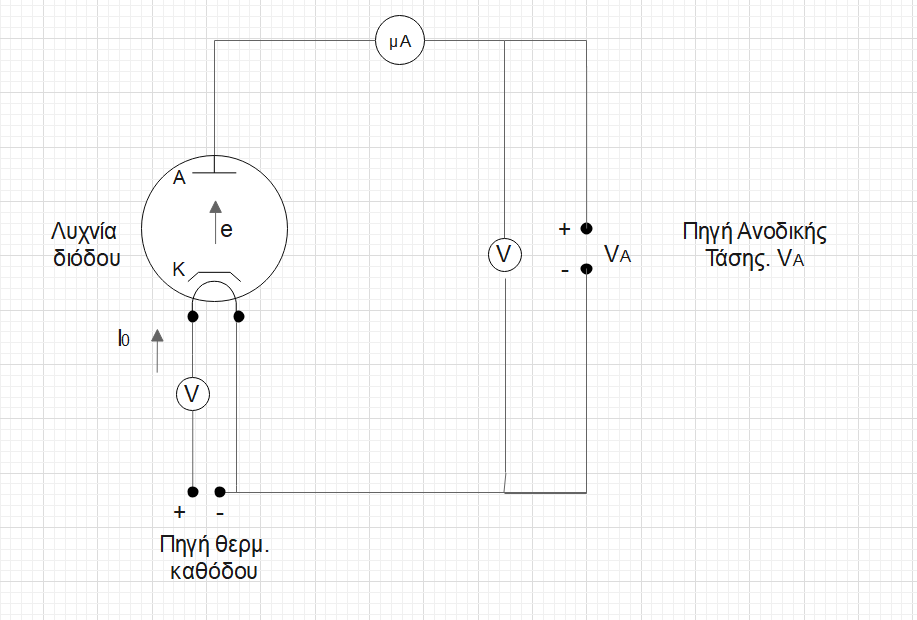
\includegraphics[scale=0.4]{circuit.png}
\end{figure}

\subsection*{Πειρματική Διαδικασία - Επεργασία Μετρήσεων}

\subsubsection*{Νόμος Langmuir}
Αρχικά, αφού συναρμολογήσουμε το ηλεκτρικό κύκλωμα της άσκησης όπως φαίνεται στην Εικόνα 2, ανοίγουμε το τροφοδοτικό. Τώρα εφαρμόζουμε στην κάθοδο ρεύμα $I_\theta = (2.267\pm 0.001)mA$ που αντιστοιχεί σε τάση θέρμανσης $V_\theta = (5.750\pm0.001)V$ και σε θερμοκρασία καθόδου $T=(2100\pm5)K$. 

Μεταβάλλουμε της τάση ανόδου $V_A = 6-20 V$ με βήμα $2V$ και καταγράφουμε την τιμή του ρεύματος ανόδου. Τα αποτελέσματα φαίνονται στον Πίνακα 1
\\
\begin{table}[h!]
\centering 
\caption{ }
\begin{tabular}{r|r|r|r|r}
\centering{\textcolor{red}{$V_A$}} & \centering{\textcolor{red}{$I_A$}}& $V_A-V_\theta/2$ & $ln(V_A-V_\theta/2)$& $ln(I_A)$\footnotemark \\ 
\textcolor{red}{$(\pm10^{-3}V)$}  & \textcolor{red}{$(\pm10^{-3}mA)$} &                  &                     &           \\
\hline\hline
%6&0.03&3.125&1.1394&-3.5066\\ 
%8&0.05&5.125&1.6341&-2.9957\\ 
%10&0.07&7.125&1.9636&-2.6593\\ 
%12&0.09&9.125&2.2110&-2.4079\\ 
%14&0.11&11.125&2.4092&-2.2073\\ 
%16&0.13&13.125&2.5745&-2.0402\\ 
%18&0.16&15.125&2.7163&-1.8326\\ 
%20&0.18&17.125&2.8405&-1.7148
6&0.03&3.125&1.1394&3.4012\\ 
8&0.05&5.125&1.6341&3.9120\\ 
10&0.07&7.125&1.9636&4.2485\\ 
12&0.09&9.125&2.2110&4.4998\\ 
14&0.11&11.125&2.4092&4.7005\\ 
16&0.13&13.125&2.5745&4.8675\\ 
18&0.16&15.125&2.7163&5.0752\\ 
20&0.18&17.125&2.8405&5.1930
\end{tabular}
\end{table}
 \footnotetext{Πρώτα μετατρέπω το $I_A$ σε Ampere.}
 \\
 Τα δεδομένα των δύο τελευταίων στηλών μας χρησιμεύουν καθώς από την σχέση (\ref{4}) έχουμε ότι 
 \begin{align*}\label{7}
 ln(I_A) = ln(B) + (3/2) \cdot  ln(V_A) \numberthis 
 \end{align*}
Συνεπώς αν θεωρήσουμε $Y=ln(I_A)$ και $X=ln(V_A)$, τότε η θεωρία προβλέπει ότι πρέπει να συνδέονται γραμμικά σύμφωνα μία σχέση της μορφής $Y=D\cdot X + C$. Έτσι, αν εφαρμόσουμε την μέθοδο ελαχίστων τετραγώνων για τα δεδομένα $X,Y$ μπορούμε να προβλέψουμε στα πλάσια κάποιου σφάλματος τον συντελεστή $D$, ο οποίος είναι ο εκθέτης στον νόμο του Langmuir και μέσω του $C=ln(B)$, να εκτιμήσουμε το Β, το οποίο είναι μία σταθερά της διάταξης. Χρησιμοποιώντας τις σχέσεις της μεθόδου ελαχίστων τετραγώνων παίρνουμε για τους συντελεστές και τα σφάλματά τους: 
\begin{align*}
D &= (1.05\pm0.01) \numberthis \\ 
C& = (2.19\pm0.02) [S.I.]\numberthis
\end{align*}
Ως συνέπεια προκύπτει το παρακάτω γράφημα: 

\begin{figure}[h!]
\centering
\caption{ }
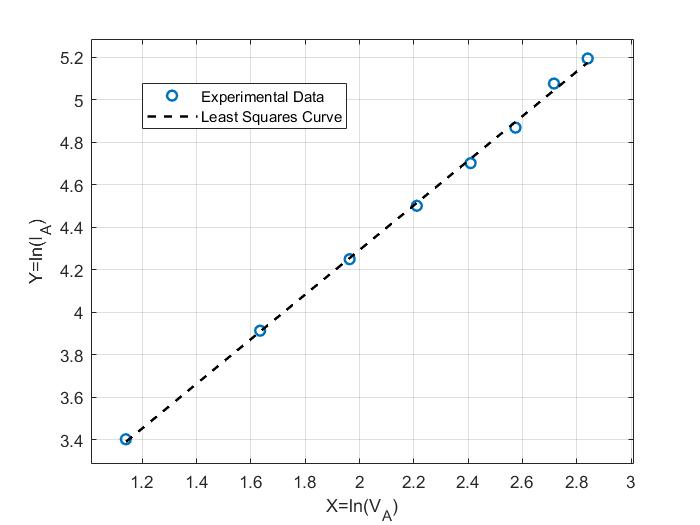
\includegraphics[scale=0.4]{Langmuir.jpg}
\end{figure}

Η τιμή του D διαφέρει κατά πολύ από την αναμενόμενη που είναι 3/2. 

Όπως παρατηρούμε από τις σχέσεις (\ref{4}) και (\ref{7}), δεν υπάρχει εισχώρηση κάποιου πειραμταικού μεγέθους στον υπολογισμό του B πέραν της τάσης $V_A$ και του ρεύματος $I_A$ της ανόδου. Ωστόσο, γνωρίζουμε πως τα σφάλματα των οργάνων είναι αρκούντως μικρά έτσι ώστε να μην δύνανται να επιδράσουν τόσο στις μετρήσεις ώστε να δώσουν μία τόσο μεγάλη απόκλιση του συντελεστή απ' το 3/2 ( έχουμε σχετικά σφάλματα $\sim 0.01\%V$ για την τάση και $\sim 1.1\%mA$ για το ρεύμα). Επίσης, δεν υπάρχει κάποιο ενδεχόμενο να έχουμε κάνει κάποιο σφάλμα κατά την διαδικασία λήψης των μετρήσεων, καθώς τα όργανα ήταν ηλεκτρονικά και δεν απαιτούνταν κάποιος χειρισμός που να βασίζεται σε δικές μας ενέργειες.

Ως εκ τούτου η αιτία του σφάλματος θα είναι κάποια αστοχία στην πειραματική διάταξη και ειδικά στην δίοδο κενού. 
%\textcolor{red}{Πιό συγκεκριμένα, για να κάνουμε την αντιστοιχία ρεύματος θέρμανσης-θερμοκρασίας της καθόδου, έχουμε θεωρήσει πως η κάθοδς έχει ευθύγραμμο και άπειρο μήκος αντί για πεπερασμένο και σε σχήμα τεθλασμένης γραμμής. Αυτή η υπόθεση δίνει τιμές της θερμοκρασίας στην κάθοδο που έιναι εν γένει μικρότερες από αυτές που χρησιμοποιούμε στην άσκηση.}
 Πιό συγκεκριμένα, η απόσταση ανόδου-καθόδου είναι πολύ μεγάλη και επίσης ο μεταλλικός δίσκος στον χώρο πίσω της καθόδου, δεν κάνει το πεδίο στον ενδιάμεσο χώρο μεταξύ καθόδου-ανόδου αρκούντως ομαλό/ομογενές, όπως έχει υποτεθεί, αλλά η μορφή του μεταβάλλεται ανάλογα με την απόσταση από την κάθοδο. Ακόμη, οι γεωμετρικές ατέλειες της λυχνίας καθώς και οι γενικότερες συνθήκες στο εργαστήριο, όπως η αυξημένη υγρασία και η πολυκαιρία των οργάνων (π.χ. εισχώρηση ατμοσφαιρικού αέρα στην λυχνία που ίσως προκαλλεί διάβρωση στα μεταλλικά στοιχεία της) ενδέχεται να συνεισφέρουν στην απόκλιση από το θεωρητικώς αναμενόμενο αποτέλεσμα.


\subsubsection*{ Σχέση Τάσης-Ρεύματος Ανόδου}
Διατηρούμε την θερμοκραία στους $T_1=(2100\pm 5)K$, δηλαδή $I_{\theta1} =(2.267\pm0.001)mA$, μεταβάλλουμε την τάση από $V_A=0-300V$ με βήμα $10V$ και καταγράφουμε την τιμή του ρεύματος με τελικό στόχο να σχεδιάσουμε την καμπύλη του ρεύματος ανόδου συναρτήσει της τάσης ανόδου. Επαναλαμβάνουμε τις μετρήσεις μας για θερμογρασίες $T_2=(2050\pm 5)K$ άρα $I_{\theta2} =(2.167\pm0.001)mA$ και $T_3=(2000\pm 5)K$ που αντιστοιχεί σε $I_{\theta3} =(2.068\pm0.001)mA$. Οι μετρήσεις φαίνονται στον Πίνακα 2.

\begin{table}[h!]
\centering
\caption{ }
\begin{tabular}{r||r|r|r}
	\toprule
\multicolumn{1}{c||}{}&\multicolumn{1}{c|}{$T_1=(2100\pm5)K$}&\multicolumn{1}{c|}{$T_2=(2050\pm 5)K$} & \multicolumn{1}{c}{$T_3=(2000\pm 5)K$} \\
%& $T_1=(2100\pm5)K$ & $T_2=(2050\pm 5)K$ & $T_3=(2000\pm 5)K$\\
	\hline
%	&	$I_{\theta1} =(2.267\pm0.0001)mA$ & $I_{\theta2} =(2.167\pm0.0001)mA$ & $I_{\theta3} =(2.068\pm0.0001)mA$\\
	 \hline
%$V_{A1}(\pm10^{-3}V)$  &  $I_{A1}(\pm10^{-3})mA$  &  $I_{A2}(\pm10^{-3})mA$  &  $I_{A3}(\pm10^{-3})mA$\\

\multicolumn{1}{c||}{$V_{A1}(\pm10^{-3}V)$}&\multicolumn{1}{c|}{$I_{A1}(\pm10^{-3})mA$}&\multicolumn{1}{c|}{$I_{A2}(\pm10^{-3})mA$} & \multicolumn{1}{c}{$I_{A3}(\pm10^{-3})mA$} \\
\hline\hline
0&0.00&0.00&0.00\\
10&0.07&0.05&0.04\\
20&0.19&0.15&0.11\\
30&0.32&0.25&0.15\\
40&0.45&0.32&0.17\\
50&0.55&0.36&0.18\\
60&0.65&0.39&0.19\\
70&0.73&0.40&0.19\\
80&0.79&0.41&0.20\\
90&0.83&0.42&0.20\\
100&0.85&0.42&0.20\\
110&0.86&0.43&0.20\\
120&0.88&0.44&0.21\\
130&0.89&0.44&0.21\\
140&0.90&0.45&0.21\\
150&0.91&0.45&0.21\\
160&0.91&0.45&0.22\\
170&0.92&0.46&0.22\\
180&0.93&0.46&0.22\\
190&0.93&0.47&0.22\\
200&0.94&0.47&0.22\\
210&0.95&0.47&0.22\\
220&0.95&0.47&0.23\\
230&0.96&0.48&0.23\\
240&0.96&0.48&0.23\\
250&0.97&0.48&0.23\\
260&0.97&0.48&0.23\\
270&0.97&0.49&0.23\\
280&0.98&0.49&0.23\\
290&0.98&0.49&0.23\\
300&-&0.49&0.24
\end{tabular}
\end{table}

Οι καμπύλες $I_{A} = I_{A}(V_A)$ με βάση τα πειραματικά δεδομένα φαίνοτναι στην Εικόνα 5.


\newpage

\begin{figure}
\centering
\caption{ }
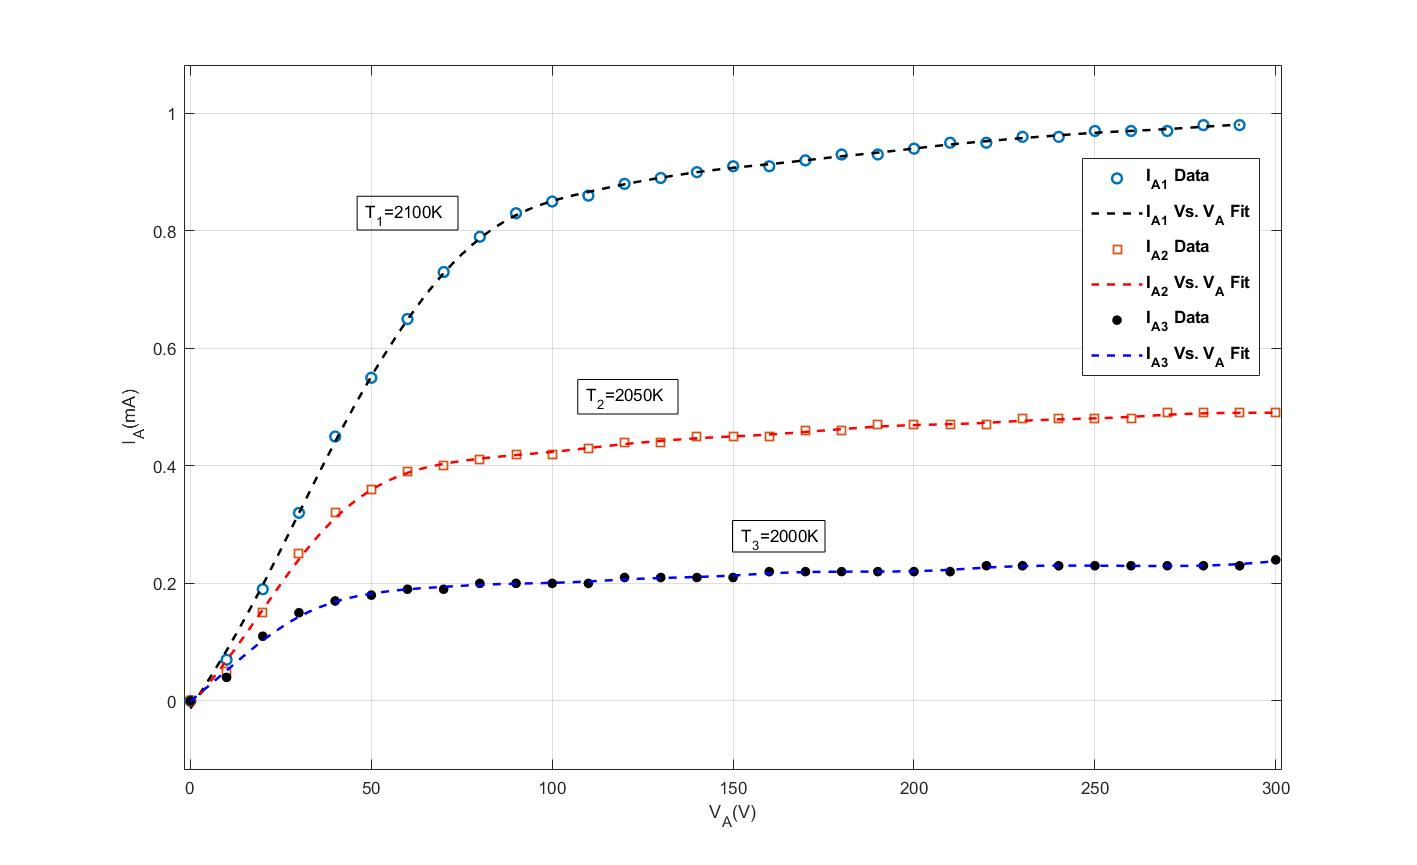
\includegraphics[scale=0.35]{i(v)_exper.jpg}
\end{figure}

Παρατηρώ ότι στις πιό υψηλές θερμοκρασίες το ρεύμα αυξάνεται αισθητά στην περιοχή του κόρου, όπου σύμφωνα με την θεωρία θα έπρεπε να είναι σχεδόν σταθερό και ανεξάρτητο από την τάση, όπως φαίνεται στην Εικόνα 2. Ακόμη, η μετάβαση στην περιοχή αυτή θα έπρεπε να είναι πιό απότομη. Η απουσία της απότομης μετάβασης στον κορεσμό, οφείλεται στο γεγονός ότι το ηλεκτρικό πεδίο της ανόδου αλληλεπιδρά πιό έντονα με την πλευρά της καθόδου που βρίσκεται κοντά του. Έτσι, το ρεύμα που προέρχεται από ηλεκτρόνια της "μπροστινής" περιοχής σταθεροποιείται πίο γρήγορα από εκείνο που οφείλεται στα ηλεκτρόνια που εξέρχονται από την "πίσω" περιοχή της καθόδου. Συνεπώς, το ένα μέρος του ρεύματος φτάνει στον κορεσμό πίο γρήγορα από το άλλο και γι' αυτό ο συνολικός κορεσμός επέρχεται πιό ομαλά και για μεγαλύτερες τάσεις από τις αναμενόμενες.


\subsubsection*{Έλεγχος του νόμου Richardson}
Σε αυτό το μέρος θα μελετηθεί το σημείο κορεσμού του ανοδικού ρεύματος.

Ορίζουμε την τάση στα 300V και καταγράφουμε τις τιμές του ανοδικού ρεύματος $I_A$ μεταβάλλοντας την θερμοκρασία της καθόδου από $T=2100-1700K$ με βήμα 50Κ. Η θερμοκρασία ρυθμίζεται μέσω της τιμής του ρεύματος καθόδου. Η σχέση των δύο αυτών μεγεθών είναι γνωστή και φαίνεται στις δύο πρώτες στήλες του Πίνακα 3, στον οποίο καταγράφονται και οι υπόλοιπες μετρήσεις.
\begin{table}[h!]
\centering
\caption{ }
\begin{tabular}{r|r||r|r|r|r}
$T(\pm5K)$ & $I_\theta(A)$ & $I_A(\pm10^{-3}mA)$ & $1/T(10^{-4}K^{-1})$ & $I_A/T^2(10^{-5}AK^{-2})$\footnotemark & $ln(I_A/T^2)$ \\ 
\hline\hline
%1700&1.512&0.001&0.000588&3e-10&-21.7845\\
%1750&1.602&0.003&0.000571&1e-09&-20.7439\\
%1800&1.692&0.010&0.000556&3.1e-09&-19.5963\\
%1850&1.784&0.020&0.000541&5.8e-09&-18.9579\\
%1900&1.877&0.050&0.000526&1.39e-08&-18.0950\\
%1950&1.973&0.110&0.000513&2.89e-08&-17.3584\\
%2000&2.068&0.230&0.000500&5.75e-08&-16.6715\\
%2050&2.167&0.490&0.000488&1.166e-07&-15.9645\\
%2100&2.267&0.980&0.000476&2.222e-07&-15.3196
1700&1.512&0.001&5.88&0.04&-14.8768\\
1750&1.602&0.003&5.71&0.10&-13.8361\\
1800&1.692&0.01&5.56&0.31&-12.6885\\
1850&1.784&0.02&5.41&0.58&-12.0501\\
1900&1.877&0.05&5.26&1.39&-11.1872\\
1950&1.973&0.11&5.13&2.89&-10.4507\\
2000&2.068&0.23&5.00&5.75&-9.7637\\
2050&2.167&0.49&4.88&11.66&-9.0568\\
2100&2.267&0.98&4.76&22.22&-8.4118
\end{tabular}
\end{table}
\footnotetext{Έχω μετατρέψει το ρεύμα σε Α.}

Η χρησιμότητα των δύο τελευταίων στηλών διαφαίνεται στα παρακάτω. 
Λογαριθμίζουμε τον νόμο του Richardson, σχέση (\ref{6}): 
\begin{align*}
ln(\frac{I_A}{T^2}) = ln(C) -\frac{\phi}{k}\frac{1}{T}\Rightarrow Y = A + B\cdot X 
\end{align*}
όπου προκειμένου να γραμμικοποιήσουμε την σχέση έχουμε θέσει $Y=I_A/T^2$, $X=1/T$, $A=ln(C)$ και $B=-\phi/k$. Οι πειραματικές τιμές των X,Y φαίνονται στις δύο τελευταίες στήλες του Πίνακα 3. Έτσι, αν προσαρμόσουμε μία ευθεία με την μέθοδο των ελαχίστων τετραγώνων σε αυτά τα δεδομένα, μπορούμε να προσδιορίσουμε πειραματικά τις σταθερές A, Β και κατ' επέκταση το έργο εξαγωγής φ και την σταθερά C. Χρησιμοποιώντας τις γνωστές σχέσεις για την μέθδο των ελαχίστων τετραγώνων προκύπτουν οι παρακάτω τιμές και η γραφική παράσταση στην Εικόνα 6: 
\begin{align*}
A &= (18.77\pm0.52)[S.I.] \numberthis \\
B &= (-5.70\pm0.10)\times10^4[S.I.] \numberthis
\end{align*}

\begin{figure}[h!]
\centering
\caption{ }
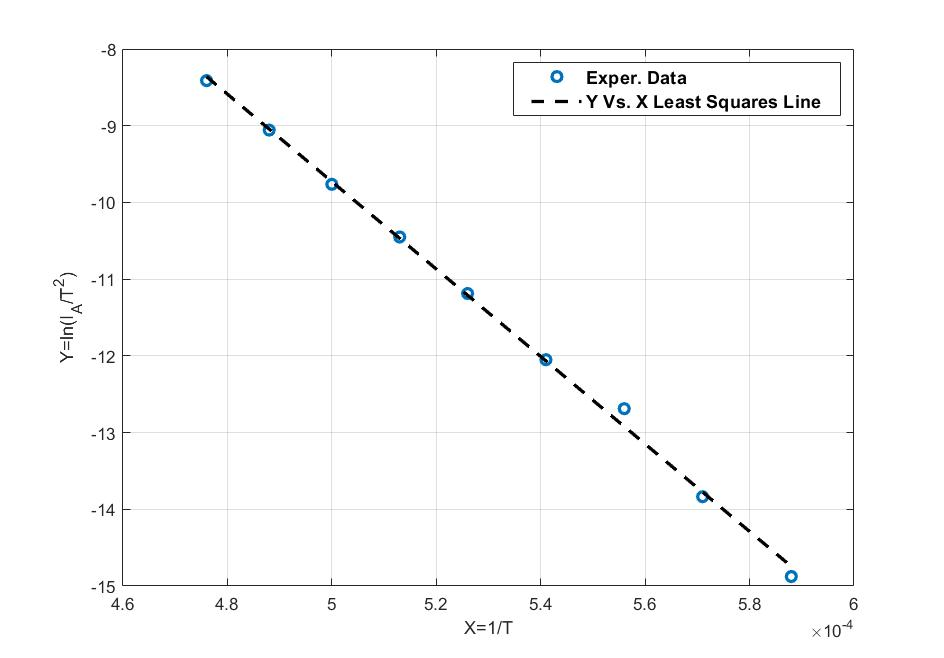
\includegraphics[scale=0.35]{richard.jpg}
\end{figure}

Άρα, από την κλίση έχουμε 
\vspace{-0.1in}
\begin{align*}
\phi =-k B = 5.70\times10^4\cdot 8.62\times10^{-5}=4.19eV
\end{align*}
Για το σφάλμα από διάδοση έχουμε 
\begin{align*}
\delta\phi = | \pdv{\phi}{B}\delta B |=|-k\delta B|=8.62\times10^{-5}\cdot 0.1\times10^{4} = 0.09eV
\end{align*}
Άρα 
\vspace{-0.2in}
\begin{align*}
\phi = (4.19\pm0.09)eV 
\end{align*}
Το αποτέλεσμα δεν περιλαμβάνει στα όρια το σφάλματός του την αναμενόμενη τιμή $4.5eV$.
Όμως, δεν έχουμε λάβει υπόψιν το φαινόμενο Schottky κατά το οποίο αν έχουμε ηλεκτρικό πεδίο της τάξης $\sim10^7V/m$ στην επιφάνεια του μετάλλου, το έργο εξαγωγής μειώνεται κατά $0.12eV$. Αν το συμπεριλάβουμε, τότε το έργο εξαγωγής γίνεται $$\phi=(4.31\pm0.09)eV$$ και προσεγγίζει περισσότερο την τιμή των $4.5eV$ που περιμένουμε.
%Η αποδεκτή τιμή για το εν λόγω έργο εξαγωγής είναι $4.5eV$ και παρατηρούμε πως αυτή που υπολογίσαμε δεν συμπίπτει με την αποδεκτή ούτε στα όρια του σφάλματός της.
Ωστόσο, επειτα από την διόρθωση, πάλι το αναμενόμενο αποτέλεσμα δεν ανήκει στα όρια του σφάλματος.
Αυτό ίσως οφείλεται στο γεγονός ότι έχουμε θεωρήσει πως τα ηλεκτρόνια εξέρχονται με ακριβώς μηδενική ταχύτητα, δηλαδή με μηδενική ενέργεια, πράγμα που δεν ισχύει απολύτως καθώς ενδέχεται να έχουν προσλάβει και μεγαλύτερα ποσά ενέργειας.


\subsection*{Συμπεράσματα}
Εν κατακλείδι, τα συμπεράσματα σε μία πρώτη ματιά είναι θετικά καθώς έχουμε αναπαράγει επιτυχώς τα ποιοτικά στοιχεία των θεωρητικώς αναμενόμενων αποτελεσμάτων. Σε επόμενη ματιά, τα ποσοτικά αποτελέσματα δεν συμπίπτουν με τα θεωρητικά ούτε στα πλαίσια των σφαλμάτων τους και απέχουν από αυτά περίπου $\sim30\%$ για τον εκθέτη του νόμου Langmuir $\sim4\%$ για το έργο εξαγωγής. Οι εν λόγω αποκλίσεις οφείλονται, όπως έχει αναφερθεί, τόσο σε θεωρητικές, όσο και σε πειραματικές αστοχίες. 

\subsection*{Βιβλιογραφία-Εργαλεία}
\begin{itemize}
\item[.] ΕΡΓΑΣΤΗΡΙΑΚΕΣ ΑΣΚΗΣΕΙΣ ΦΥΣΙΚΗΣ ΤΟΜΟΣ ΙΙ, ΣΥΛΛΟΓΙΚΟ
\item[.] Matlab για επεξαργασία $\&$ γραφικές παραστάσεις
\item[.] EdrawMax για τα σχήματα
\end{itemize}
\end{document}